\documentclass[12pt]{article}

\usepackage{amsmath, mathtools}
\usepackage{amsfonts}
\usepackage{amssymb}
\usepackage{graphicx}
\usepackage{colortbl}
\usepackage{xr}
\usepackage{hyperref}
\usepackage{longtable}
\usepackage{xfrac}
\usepackage{tabularx}
\usepackage{float}
\usepackage{siunitx}
\usepackage{booktabs}
\usepackage{caption}
\usepackage{pdflscape}
\usepackage{afterpage}
\usepackage{graphicx}
\usepackage{float}

\usepackage[round]{natbib}

%\usepackage{refcheck}

\hypersetup{
    bookmarks=true,         % show bookmarks bar?
    colorlinks=true,        % false: boxed links; true: colored links
    linkcolor=red,          % color of internal links (change box color with linkbordercolor)
    citecolor=green,        % color of links to bibliography
    filecolor=magenta,      % color of file links
    urlcolor=cyan           % color of external links
}

%% Comments

\usepackage{color}

\newif\ifcomments\commentstrue %displays comments
%\newif\ifcomments\commentsfalse %so that comments do not display

\ifcomments
\newcommand{\authornote}[3]{\textcolor{#1}{[#3 ---#2]}}
\newcommand{\todo}[1]{\textcolor{red}{[TODO: #1]}}
\else
\newcommand{\authornote}[3]{}
\newcommand{\todo}[1]{}
\fi

\newcommand{\wss}[1]{\authornote{blue}{SS}{#1}} 
\newcommand{\plt}[1]{\authornote{magenta}{TPLT}{#1}} %For explanation of the template
\newcommand{\an}[1]{\authornote{cyan}{Author}{#1}}

%% Common Parts

\newcommand{\progname}{ProgName} % PUT YOUR PROGRAM NAME HERE
\newcommand{\authname}{Team \#, Team Name
\\ Student 1 name
\\ Student 2 name
\\ Student 3 name
\\ Student 4 name} % AUTHOR NAMES                  

\usepackage{hyperref}
    \hypersetup{colorlinks=true, linkcolor=blue, citecolor=blue, filecolor=blue,
                urlcolor=blue, unicode=false}
    \urlstyle{same}
                                


% For easy change of table widths
\newcommand{\colZwidth}{1.0\textwidth}
\newcommand{\colAwidth}{0.13\textwidth}
\newcommand{\colBwidth}{0.82\textwidth}
\newcommand{\colCwidth}{0.1\textwidth}
\newcommand{\colDwidth}{0.05\textwidth}
\newcommand{\colEwidth}{0.8\textwidth}
\newcommand{\colFwidth}{0.17\textwidth}
\newcommand{\colGwidth}{0.5\textwidth}
\newcommand{\colHwidth}{0.28\textwidth}

% Used so that cross-references have a meaningful prefix
\newcounter{defnum} %Definition Number
\newcommand{\dthedefnum}{GD\thedefnum}
\newcommand{\dref}[1]{GD\ref{#1}}
\newcounter{datadefnum} %Datadefinition Number
\newcommand{\ddthedatadefnum}{DD\thedatadefnum}
\newcommand{\ddref}[1]{DD\ref{#1}}
\newcounter{theorynum} %Theory Number
\newcommand{\tthetheorynum}{T\thetheorynum}
\newcommand{\tref}[1]{T\ref{#1}}
\newcounter{tablenum} %Table Number
\newcommand{\tbthetablenum}{T\thetablenum}
\newcommand{\tbref}[1]{TB\ref{#1}}
\newcounter{assumpnum} %Assumption Number
\newcommand{\atheassumpnum}{P\theassumpnum}
\newcommand{\aref}[1]{A\ref{#1}}
\newcounter{goalnum} %Goal Number
\newcommand{\gthegoalnum}{P\thegoalnum}
\newcommand{\gsref}[1]{GS\ref{#1}}
\newcounter{instnum} %Instance Number
\newcommand{\itheinstnum}{IM\theinstnum}
\newcommand{\iref}[1]{IM\ref{#1}}
\newcounter{tdreqnum} %Tray Dispensing Requirement Number
\newcommand{\rthetdreqnum}{P\thetdreqnum}
\newcommand{\tdrref}[1]{TDR\ref{#1}}
\newcounter{pdreqnum} %Pot Dispensing Requirement Number
\newcommand{\rthepdreqnum}{P\thepdreqnum}
\newcommand{\pdrref}[1]{PDR\ref{#1}}
\newcounter{creqnum} %Conveyor Requirement Number
\newcommand{\rthecreqnum}{P\thecreqnum}
\newcommand{\crref}[1]{CR\ref{#1}}
\newcounter{vreqnum} %Verification Requirement Number
\newcommand{\rthevreqnum}{P\thevreqnum}
\newcommand{\vrref}[1]{VR\ref{#1}}
\newcounter{nfrnum} %NFR Number
\newcommand{\rthenfrnum}{NFR\thenfrnum}
\newcommand{\nfrref}[1]{NFR\ref{#1}}
\newcounter{lcnum} %Likely change number
\newcommand{\lthelcnum}{LC\thelcnum}
\newcommand{\lcref}[1]{LC\ref{#1}}
\newcounter{reqnum} %Requirement Number
\newcommand{\rthereqnum}{P\thereqnum}
\newcommand{\rref}[1]{R\ref{#1}}
\newcounter{lctdreqnum} %Likely change number
\newcommand{\lthelctdreqnum}{LC\thelctdreqnum}
\newcommand{\lctdref}[1]{TDR\ref{#1}}
\newcounter{lcpdreqnum} %Likely change number
\newcommand{\lthelcpdreqnum}{LC\thelcpdreqnum}
\newcommand{\lcpdref}[1]{PDR\ref{#1}}
\newcounter{lccreqnum} %Likely change number
\newcommand{\lthelccreqnum}{LC\thelccreqnum}
\newcommand{\lccref}[1]{CR\ref{#1}}
\newcounter{lcvreqnum} %Likely change number
\newcommand{\lthelcvreqnum}{LC\thelcvreqnum}
\newcommand{\lcvref}[1]{VR\ref{#1}}

\usepackage{fullpage}

\newcommand{\deftheory}[9][Not Applicable]
{
\newpage
\noindent \rule{\textwidth}{0.5mm}

\paragraph{RefName: } \textbf{#2} \phantomsection 
\label{#2}

\paragraph{Label:} #3

\noindent \rule{\textwidth}{0.5mm}

\paragraph{Equation:}

#4

\paragraph{Description:}

#5

\paragraph{Notes:}

#6

\paragraph{Source:}

#7

\paragraph{Ref.\ By:}

#8

\paragraph{Preconditions for \hyperref[#2]{#2}:}
\label{#2_precond}

#9

\paragraph{Derivation for \hyperref[#2]{#2}:}
\label{#2_deriv}

#1

\noindent \rule{\textwidth}{0.5mm}

}

\begin{document}

\title{Software Requirements Specification for The Nursery Project: The Pot-Pulator} 
\author{\authname}
\date{\today}
	
\maketitle

~\newpage

\pagenumbering{roman}

\tableofcontents

~\newpage

\section*{Revision History}

\begin{tabularx}{\textwidth}{p{3cm}p{2cm}X}
\toprule {\bf Date} & {\bf Version} & {\bf Notes}\\
\midrule
Date 1 & 1.0 & Notes\\
Date 2 & 1.1 & Notes\\
\bottomrule
\end{tabularx}

~\newpage

\section{Reference Material}

This section records information for easy reference.

\subsection{Table of Units}

Throughout this document SI (Syst\`{e}me International d'Unit\'{e}s) is employed
as the unit system.  In addition to the basic units, several derived units are
used as described below.  For each unit, the symbol is given followed by a
description of the unit and the SI name.
~\newline

\renewcommand{\arraystretch}{1.2}
%\begin{table}[ht]
  \noindent \begin{tabular}{l l l} 
    \toprule		
    \textbf{symbol} & \textbf{unit} & \textbf{SI}\\
    \midrule 
    \si{\metre} & length & metre\\
    \si{\kilogram} & mass	& kilogram\\
    \si{\second} & time & second\\
    \si{\celsius} & temperature & centigrade\\
    \si{\joule} & energy & joule\\
    \si{\watt} & power & watt (W = \si{\joule\per\second})\\
    \bottomrule
  \end{tabular}
  %	\caption{Provide a caption}
%\end{table}

\subsection{Table of Symbols}

The table that follows summarizes the symbols used in this document along with
their units.  The choice of symbols was made to be consistent with the heat
transfer literature and with existing documentation for solar water heating
systems.  The symbols are listed in alphabetical order.

\renewcommand{\arraystretch}{1.2}
%\noindent \begin{tabularx}{1.0\textwidth}{l l X}
\noindent \begin{longtable*}{l l p{12cm}} \toprule
\textbf{symbol} & \textbf{unit} & \textbf{description}\\
\midrule 
$A_C$ & \si[per-mode=symbol] {\square\metre} & coil surface area
\\
$A_\text{in}$ & \si[per-mode=symbol] {\square\metre} & surface area over 
which heat is transferred in
\\ 
\bottomrule
\end{longtable*}

\subsection{Abbreviations and Acronyms}

\renewcommand{\arraystretch}{1.2}
\begin{tabular}{l l} 
  \toprule		
  \textbf{symbol} & \textbf{description}\\
  \midrule 
  A & Assumption\\
  DD & Data Definition\\
  GD & General Definition\\
  GS & Goal Statement\\
  IM & Instance Model\\
  LC & Likely Change\\
  PS & Physical System Description\\
  R & Requirement\\
  SRS & Software Requirements Specification\\
  \progname{} & \\
  T & Theoretical Model\\
  \bottomrule
\end{tabular}\\

\subsection{Mathematical Notation}

\newpage

\pagenumbering{arabic}


\section{Introduction}

The current method of preparing pots and trays to be filled with soil and populated with seeds at Sheridan Nurseries is a process with little to no automation, requiring many manual labour hours. Each year, 250,000 pots need to be placed in trays, each one being placed by hand. Recently, the owners of these farms have been finding it increasingly more difficult to fill these roles with enough workers to run the operation smoothly and meet production demands.\\

\noindent We aim to aid in this process by designing and implementing a machine that is able to fill trays with pots and prepare them for populating with soil and seeds. This will alleviate the reliance on manual labour and improve the overall efficiency of the farm. \\

\noindent This introduction will outline the document’s purpose, the scope of requirements, characteristics of the intended reader, and the organization of document. 


\subsection{Purpose of Document}

This Software Requirements Specification (SRS) document is to define the purpose of the Pot-Pulator. It will describe how the software will interact with the hardware, and how it is expected to perform, defining the executable requirements leading to the creation of a final product. This document should lay the important groundwork needed for every team member to understand the in-depth technical details of the product to be developed, in preparation for the design stage. 

\subsection{Scope of Requirements} 

The branches of the Pot-Pulator include a conveyer belt, tray allocation, pot dropping and verification. These four systems will be implemented to work together to create an efficient product. It will be reliable, easily configurable, affordable, and will greatly reduce the need for hands-on labour in relation to seed population.  \\

\noindent The system implemented will be designed exclusively for Sheridan Nurseries, and for the pots and trays at their locations in a three-dimensional workspace. It is limited to usage on their round, 4-inch diameter pots and their respective trays. Considering the conditions of the greenhouses this machine will be used in, material degradation, water resistance, and pressure will all be negligible. \\

\noindent In order to maintain speed of the pots being placed in trays in a timely manor, one of the goals of the machine is to fill each tray with 10 pots every 30 seconds. This is the time it will take for the trays to be populated and move down the conveyer belt. With this goal in place, the machine will only need to be refilled with pots and trays every 15 minutes, greatly reducing the amount of hands-on labour from the workers at Sheridan Nurseries. \\

\noindent After the initial completion of the goal associated with the 4-inch pots, larger pots and trays may be considered as a future goal. There will always be the limitation of the requirement of a rim on the top of the pot, for the machine to easily grasp onto when lifting and dropping. \\


\subsection{Behavioural Overview}
The Pot-Pulator will have 4 branches working together to accomplish the task. First, the trays and pots will be manually filled into a section of the machine, ideally 30 trays and 300 pots. The first section of the machine will drop a tray, and the conveyer belt will move it to the pot dropping section. \\

\noindent The conveyer belt will stop once it senses the tray is in the correct position. The machine will drop pots until all 10 spots are filled. The conveyer belt will move the tray according to the needed positions for pot dropping, dispensing 2 pots into the allocated positions, moving forward 4 inches at a time until the process is completed. \\

\noindent The tray filled with pots will then move into a verification system, to verify the pots have been placed in the correct positions. The conveyer belt will then move it to an existing conveyer system, which will lead to the collection of completed trays. The only maintenance this machine needs is the refill of pots and trays every 15 minutes, and the collection of completed trays at the end of the final conveyer belt. \\

\subsection{Clients and Stakeholders}
\noindent This system provides a solutuion for all nursery applications that are not working on the cutting edge. For those nurseries that have an existing assembly line to fulfil their propagation this is a great solution as other solutions repolace the assembly line in its entirity, this solution instead adds to it.
\noindent Clients include:
\begin{itemize}
    \item Sheridan Nurseries manager
    \item Sheridan Nurseries owner
\end{itemize}
\noindent Stakeholders include:
\begin{itemize}
    \item Dr. Smith (Project Supervisor).
    \item Juan Moncada, Gillian Ford, Aaron Billiones, and Steven Ramundi, (Project Proposers).
    \item Nicholas Annable (Supervising TA)
    
\end{itemize}


\subsection{Characteristics of Intended Reader} \label{sec_IntendedReader}

This SRS document is written for the individuals directly involved with the development of the Pot-Pulator. This includes every member of the team; all being involved with the development of the project. It is useful as reference to the functionality of in-depth details regarding the project, and will be read, reviewed, and maintained as the project progresses by all team members. \\

\noindent In general, any users of this document should have an undergraduate level understanding of software and hardware system functionality, physics, and mathematics. \\

\subsection{Organization of Document}

This SRS template is based on \citet{SmithAndLai2005, SmithEtAl2007}. These templates have been modified to reflect rubric requirements, and sections have been reorganized to follow 
the LazyBots student sample SRS. Sections 3 and 4 describe the project constraints, and show the context and functional decomposition diagrams. 
Section 5 is dedicated to functional requirements. This section will define functional requirements seperated in terms of the systems which make up the Pot-Pulator. 
Section 6 describes the non-functional requirements in terms of look and feel, usability, performance, operational, maintainability and portability, security, cultural and political, 
and legal requirements. Section 7 evaluates each functional requirement on its likelihood to change, and specifies how the requirement may change if it is not very unlikely to.


\section{Project Constraints}

This section identifies the
interfaces between the system and its environment, describes the user
characteristics, lists the system constraints, and provides assumptions relating to the system/environment.

\subsection{System Context}
The system will consist of a stack of pots, stack of trays, and the mechanism that will 
autonomously populate the trays with the pots. The trays will move along a conveyor system that operates at approximately 3 feet 
and will act as the operating workspace for the device. Once the trays are populated with pots,
they are fed into a soil potting machine in preparation for planting.

\subsection{User Responsibilities \& Characteristics}

The user will be responsible for refilling the stacks of trays and pots when the supply is depleted. 
The user will also be responsible for knowing how the entire system will operate within each state. 
For example, if a tray fails the validation step, the user must be capable of removing the defect and resume the operation of the machine.\\\\
\noindent The characteristics of the user will ensure smooth operation and workplace safety. The user should be 
able to lift a sufficient weight and have a good understanding of basic functionality of the system.


\subsection{System Constraints}

The system constraints are in place to comply with the physical and 
technical limits provided to the team.

\subsubsection{Physical Constraints}
\begin{tabular}{ |p{2cm}|p{14cm}| }
  \hline
  PHC0 & Workspace dimensions (including stacks of 
  trays and pots) of height = 12' width = 6' length = 8'\\
  \hline
  Rationale & the allowable workspace area provided by Sheridan Nurseries  \\ 

  \hline  
 \end{tabular}\\\\

 \noindent
 \begin{tabular}{ |p{2cm}|p{14cm}| }
  \hline
  PHC1 & Conveyor system must be height = 3'  
  width = 1.5' length = 8' (maximum) \\
  \hline
  Rationale & the new system will feed trays into an existing soil potting 
  machine via conveyor system so they must operate in a similar manner  \\ 

  \hline  
 \end{tabular}\\\\

 \noindent
 \begin{tabular}{ |p{2cm}|p{14cm}| }
  \hline
  PHC2 & Operational in winter temperatures (outdoor conditions)  \\
  \hline
  Rationale & operation takes place in a 
  tent outside between January and February  \\ 

  \hline  
 \end{tabular}\\\\

 \noindent
 \begin{tabular}{ |p{2cm}|p{14cm}| }
  \hline
  PHC3 & Fully operational through a standard 3-prong 120V wall outlet   \\
  \hline
  Rationale & the system’s environment requires this 
  as the only source of power  \\ 

  \hline  
 \end{tabular}\\\\
 
  
\subsubsection{Software Constraints}
\begin{tabular}{ |p{2cm}|p{14cm}| }
  \hline
  SWC0 & Perform operations and calculations in a timely manner \\
  \hline
  Rationale &  to ensure the system can actually replace a human  \\ 

  \hline  
 \end{tabular}\\\\

 \subsection{Assumptions}
 The following assumptions are being made when designing and developing 
  the device:
 \begin{itemize}
  
  \item The user will fill the machine with stacks of trays and 
  pots as required

  \item The system will populate 10 pots of 4-inch diameter into its 
  respective tray
  \item The system can hold stacks sufficient enough for 15-30 minutes of continuous operation
  
 \end{itemize}

 \subsection{Constants}
 \begin{tabular}{ |p{4cm}|p{12cm}| }
  \hline
  Constant Name & Description\\
  \hline
  Number of Pots & The number of pots that 
  needs to be populated in a single tray\\
  \hline
  Number of Trays & The number of trays that will be populated at once \\ 
  \hline  
  Max Pots in Stack & The maximum number of 
  pots that may be stacked in the machine\\
  \hline
  Max Trays in Stack & The maximum number of 
  trays that may be stacked in the machine\\
  \hline
  Pot Size/Shape & The size/shape of the pots\\
  \hline
  Max Rate of Operation & The maximum rate at which the machine operates 
  is determined by the soil potting machine \\
  \hline
 \end{tabular}\\\\

 \subsection{Monitored Variables}
 \begin{tabular}{ |p{3cm}|p{9cm}|p{2cm}|p{1cm}| }
  \hline
  Variable & Description & Type & Units\\
  \hline
  Conveyor Speed & The speed at which the conveyor belt will move
   & Speed & m/s\\
  \hline
  Sensor Distances & Measured distances that the sensor identifies
   & Distance & mm\\
  \hline
  System State & Determines the state of the system (ie. Ready, Running, Error, Success)
   & State &  N/A\\
  \hline
  Tray/Pot Weight & Weight of the trays/pots to verify number in the stack
   & Weight & kg\\
  \hline
  Tray/Pot Height & Height of the trays/pots to verify number in the stack
   & Height & m\\
  
  \hline
 \end{tabular}\\\\

 \subsection{Controlled Variables}
 \begin{tabular}{ |p{3cm}|p{9cm}|p{2cm}|p{1cm}| }
  \hline
  Variable & Description & Type & Units\\
  \hline
  Motor Speeds & The speeds at which the motors in the system will turn
   & Speed & rad/s\\
  \hline
  Voltage in & Voltage going into the system
   & Voltage & V\\
  \hline
  Current in & Current going into the system
   & Current &  A\\
  \hline
  LEDs & LED status lights
   & Boolean & N/A\\
  
  \hline
 \end{tabular}\\\\

\subsection{Context Diagrams}
Below is a high level overview of the system. This shows all the inputs and outputs
of the overall system.

\begin{figure}[H]
  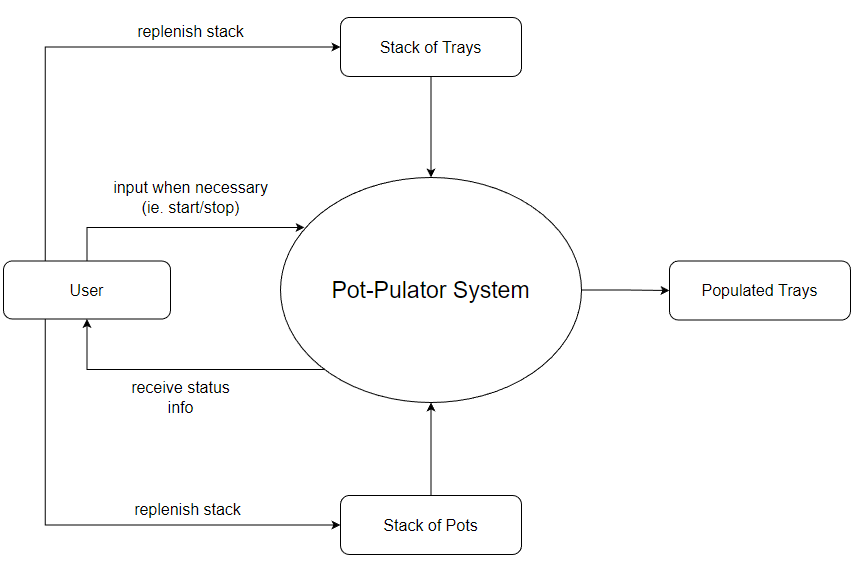
\includegraphics[width=\linewidth]{contextDiagram.png}
  \caption{Context Diagram}
  \label{fig:context1}
\end{figure}

  \section{Functional Requirements}

  This section provides the functional requirements of the Pot-Pulator, seperated into tray dispensing,
  pot dispensing, conveyor, and verification requierements.
 
  \subsection{Tray Dispensing Functional Requirements}
  
  \noindent \begin{itemize}
  
  \item[TDR\refstepcounter{tdreqnum}\thetdreqnum \label{R_Tray0}:] {The tray dispenser must
      start when the Pot-Pulator start is pressed.}
  
  \item[TDR\refstepcounter{tdreqnum}\thetdreqnum \label{R_Tray1}:] {The tray dispenser must
      be able to place a standard tray from the loaded stack onto the conveyor belt.}
  
  \item[TDR\refstepcounter{tdreqnum}\thetdreqnum \label{R_Tray2}:] {The tray dispenser must
        be able to store multiple trays at a time.}
  
  \item[TDR\refstepcounter{tdreqnum}\thetdreqnum \label{R_Tray5}:] {The tray dispenser must
      stop operating once it has run out of trays.}
  
  \item[TDR\refstepcounter{tdreqnum}\thetdreqnum \label{R_Tray6}:] {The tray dispenser must
      be able to recognize when trays need to be reloaded and notify an operator.}
  
  \item[TDR\refstepcounter{tdreqnum}\thetdreqnum \label{R_Tray7}:] {The tray dispenser must
       stop when an error arises (verification failed, pot dispenser malfunction/empty, conveyor
       malfunction).}
  
  \item[TDR\refstepcounter{tdreqnum}\thetdreqnum \label{R_Tray8}:] {The tray dispenser must
      be able to reset after it has been stopped due to error or needs to reload}
  
  
  \end{itemize}
  
  \subsection{Pot Dispensing Functional Requirements}
  
  \noindent \begin{itemize}
  
  \item[PDR\refstepcounter{pdreqnum}\thepdreqnum \label{R_Pot0}:] {The pot dispenser must
      start when the Pot-Pulator start is pressed.}
  
  \item[PDR\refstepcounter{pdreqnum}\thepdreqnum \label{R_Pot1}:] {The pot dispenser must
      be able to place a pot into an empty place in a tray.}
  
  \item[PDR\refstepcounter{pdreqnum}\thepdreqnum \label{R_Pot2}:] {The pot dispenser must
      be able to dispense a 4" diameter pot.}
  
  \item[PDR\refstepcounter{pdreqnum}\thepdreqnum \label{R_Pot3}:] {The pot dispenser must
      be able to store multiple pots at a time.}
  
  \item[PDR\refstepcounter{pdreqnum}\thepdreqnum \label{R_Pot6}:] {The pot dispenser must
      stop operating once it has run out of pots.}
  
  \item[PDR\refstepcounter{pdreqnum}\thepdreqnum \label{R_Pot7}:] {The pot dispenser must
      be able to recognize when pots need to be reloaded and notify an operator.}
  
  \item[PDR\refstepcounter{pdreqnum}\thepdreqnum \label{R_Pot8}:] {The pot dispenser must
      stop when an error arises (verification failed, tray dispenser malfunction/empty, conveyor
      malfunction).}
  
  \item[PDR\refstepcounter{pdreqnum}\thepdreqnum \label{R_Pot9}:] {The pot dispenser must
      be able to reset after it has been stopped due to an error or needs to reload.}
  
  \end{itemize}
  
  \subsection{Conveyor Requirements}
  
  \noindent \begin{itemize}
  
  \item[CR\refstepcounter{creqnum}\thecreqnum \label{R_Conveyor0}:] {The conveyor must
      start when the Pot-Pulator start is pressed.}

  \item[CR\refstepcounter{creqnum}\thecreqnum \label{R_Conveyor1}:] {The conveyor must
      be able to move a tray from the tray dispensing station to the verification station.}
  
  \item[CR\refstepcounter{creqnum}\thecreqnum \label{R_Conveyor2}:] {The conveyor must
      be able to stop when a tray is being placed on the conveyor, or when a pot is being
      placed in a tray.}
      
  \item[CR\refstepcounter{creqnum}\thecreqnum \label{R_Conveyor4}:] {The conveyor material 
      must have a high enough friction such that the trays do not slide while in contact with
      the belt.}
  
  \item[CR\refstepcounter{creqnum}\thecreqnum \label{R_Conveyor5}:] {The conveyor must
      stop when an error arises (verification failed, pot dispenser malfunction/empty, tray dispenser
      malfunction/empty).}
  \item[CR\refstepcounter{creqnum}\thecreqnum \label{R_Conveyor6}:] {The conveyor must
      be able to reset after it has been stopped due to an error or pots/trays need to
      be reloaded.}
  
  \end{itemize}
  
  \subsection{Verification Requirements}
  
  \noindent \begin{itemize}
  
  \item[VR\refstepcounter{vreqnum}\thevreqnum \label{R_Verification1}:] {The verification must
      check that only one tray is being output by the conveyer belt, and the tray is
      filled with exactly 10 pots, such that $n_{traysout}=1\ \&\ n_{potsout}=10$}
  
  \item[VR\refstepcounter{vreqnum}\thevreqnum \label{R_Verification2}:] {The verification must
      notify all other systems if verification failes, such that $n_{traysout}\neq1\ or\ n_{potsout}\neq10$}
  
  \end{itemize}
  
  
  
  
  \section{Nonfunctional Requirements}
  the systems nonfunctional requirements will be divided by categories for which the requirements fit into. The mention of subsystems
  throughout this section is a reference to the four subsystems that the project can be devided into; conveyor, tray dispenser, pot dispenser and verification.
  
  \subsection{Appearance Requirements}

  \noindent 
  \begin{itemize}
  
  \item[NFR\refstepcounter{nfrnum}\thenfrnum \label{NFR_Accuracy}:]
    All electrical equipment and electronics must be well covered and protected. The User must not have access to equipment.
  
  \item[NFR\refstepcounter{nfrnum}\thenfrnum \label{NFR_Usability}:]
    All wiring must be tucked away and not accessible to avoid potential woring failure.
  
  \item[NFR\refstepcounter{nfrnum}\thenfrnum \label{NFR_Maintainability}:]
    All moviung part must be covered and protected. moving parts should be covered to protect both the mechanism and the safety of the opperator.

  \end{itemize}
  
  \subsection{Usability Requirements}

  \noindent \begin{itemize}
  
  \item[NFR\refstepcounter{nfrnum}\thenfrnum \label{NFR_Portability1}:]
  System must have tray and pot refill locations visible and accessible in order to provide visual verification of capacity status.
  
  \item[NFR\refstepcounter{nfrnum}\thenfrnum \label{NFR_Portability2}:]
  System output (end of conveyor) must be clear and visible in order to provide visual verification and access to failed outputs.
  \end{itemize}
  \subsection{Learning Requirments}

  \noindent \begin{itemize}
  \item[NFR\refstepcounter{nfrnum}\thenfrnum \label{NFR_Portability3}:]
  System must be simple to opperate, requiiring minimal training to opperate effectively ($<1h$).

  \end{itemize}


  \subsection{Accessibility Requirements}
 \noindent \begin{itemize}
  \item[NFR\refstepcounter{nfrnum}\thenfrnum \label{NFR_Portability4}:]
  System must have both audible and visible signal outputs for each system status.
 \end{itemize}

  \subsection{Speed Requirements}
  \noindent \begin{itemize}
  \item[NFR\refstepcounter{nfrnum}\thenfrnum \label{NFR_Portability5}:]
  Conveyor system must not accelerate in a manner that would hsift the position of the tray. a shift in the position of the tray could result in a misalignement and potential error.
  
  \item[NFR\refstepcounter{nfrnum}\thenfrnum \label{NFR_Portability6}:] 
  {The pot dispenser must 
  dispense pots at a rate of 10 pots every 30 seconds, such that $t_{cycle}=30\ seconds
      \ \&\ n_{pots}\left(t\right)=300-t/3;\ t\ \varepsilon\ \{30, 60, 90, ..., 900\}$}
  This will allow the machine to meet the output goal required.
  \end{itemize}  


  \subsection{Safety Critical Requirements}
  \noindent \begin{itemize}
  \item[NFR\refstepcounter{nfrnum}\thenfrnum \label{NFR_Portability7}:]
  System must hgave emergency cut off. in case of any emergency this will trip off all power to system.
  
  \item[NFR\refstepcounter{nfrnum}\thenfrnum \label{NFR_Portability8}:]
  System must be able to locate and identify failures  within each independent subsystem.
  
  \end{itemize}
  \subsection{Precision Requirements}
  \noindent \begin{itemize}
  \item[NFR\refstepcounter{nfrnum}\thenfrnum \label{NFR_Portability9}:]
  Conveyor must center trays before potting dispensor withing 1 cm of centered position, this allows the tray to enter the pot dispensing system within tolerance for a pot to be dropped in.
  \end{itemize}


  \subsection{Capacity Requirements}
  \noindent \begin{itemize}
  \item[NFR\refstepcounter{nfrnum}\thenfrnum \label{NFR_Portability10}:] {The pot dispenser must
  be able to take a maximum of 30 pots from the user, such that 
  $n_{pots}(t)\le300$} 
  This will allow the machine to meet the output goal required.


  \item[NFR\refstepcounter{nfrnum}\thenfrnum \label{NFR_Portability11}:]
  Pot dispensor should dispence pots within a 0.5 cm radius of centered position.
  \end{itemize}


  \subsection{Reliability Requirements}
  \noindent \begin{itemize}
  \item[NFR\refstepcounter{nfrnum}\thenfrnum \label{NFR_Portability12}:]
  System must be able to opperate under constant low and high frequency vibration (small amplitude).
  
  \end{itemize}


  \subsection{Robustness and Fault Tolerance Requirements}
  \noindent \begin{itemize}
  \item[NFR\refstepcounter{nfrnum}\thenfrnum \label{NFR_Portability19}:]
  Components must withstand 250,000 cycles system should call for replacement parts after a full season of opperation.
  
  \end{itemize}

  \subsection{Scalability or Extensibility Requirements}
  \noindent \begin{itemize}
  \item[NFR\refstepcounter{nfrnum}\thenfrnum \label{NFR_Portability20}:]
  System must fit into the existing assembly line and should take minimal effort to implement ($<1d$).
  \end{itemize}


  \subsection{Expected Physical Environement Requirements}
  \noindent \begin{itemize}
  \item[NFR\refstepcounter{nfrnum}\thenfrnum \label{NFR_Portability13}:]
  System must withstand operating in a room with high arial polution including dust, dirt and small amounts of water.
  \end{itemize}
  \subsection{Maitenance Requirements}
  \noindent \begin{itemize}
  \item[NFR\refstepcounter{nfrnum}\thenfrnum \label{NFR_Portability14}:]
  System must be built for ease of maitenance. high wear parts should be easily accessible.
  \end{itemize}


  \subsection{Requirements for Interacting with Adjacent Systems }\
  \noindent \begin{itemize}
  \item[NFR\refstepcounter{nfrnum}\thenfrnum \label{NFR_Portability15}:]
  system must opperate at same speed as adjacent systems.
  
  \item[NFR\refstepcounter{nfrnum}\thenfrnum \label{NFR_Portability16}:]
  System must opperate at the same conveyor height as the current system to maintain continuity between systems.
  
  \end{itemize}

  \subsection{Supportability Requirements }\
  \noindent \begin{itemize}
  \item[NFR\refstepcounter{nfrnum}\thenfrnum \label{NFR_Portability17}:]
  System documentation must be available to troubleshoot, diagnose and fix common issues and replace high wear parts.
  \end{itemize}

  \subsection{Compliance Requirements }\
  \noindent \begin{itemize}
  \item[NFR\refstepcounter{nfrnum}\thenfrnum \label{NFR_Portability18}:]
  System must follow electronics system safety requirements.
  \end{itemize}
  

\section{Functional Requirements Likelihood of Change}

\subsection{Tray Dispensing Functional Requirements}

\noindent \begin{itemize}

\item[TDR\refstepcounter{lctdreqnum}\thelctdreqnum\label{LC_meaningfulLabel0}:] {Very unlikely to change,
    key implementation of system.}

\item[TDR\refstepcounter{lctdreqnum}\thelctdreqnum\label{LC_meaningfulLabel1}:] {Very unlikely to change,
    key implementation of system.}

\item[TDR\refstepcounter{lctdreqnum}\thelctdreqnum\label{LC_meaningfulLabel2}:] {Very unlikely to change,
    key implementation of system.}

\item[TDR\refstepcounter{lctdreqnum}\thelctdreqnum\label{LC_meaningfulLabel3}:] {Very unlikely to change,
    ensures safety of operator reloading trays.}

\item[TDR\refstepcounter{lctdreqnum}\thelctdreqnum\label{LC_meaningfulLabel4}:] {Very unlikely to change,
    key implementation of system.}

\item[TDR\refstepcounter{lctdreqnum}\thelctdreqnum\label{LC_meaningfulLabel5}:] {Very unlikely to change,
    ensures safety of operator and prevents machine from dispensing trays while conveyor and/or pot dispenser
    are not operational.}

\item[TDR\refstepcounter{lctdreqnum}\thelctdreqnum\label{LC_meaningfulLabel6}:] {Unlikely to change,
    ensures safety of operator and robustness of Pot-Pulator. May change to be integrated with start
    command or resume command.}

\end{itemize}

\subsection{Pot Dispensing Functional Requirements}

\noindent \begin{itemize}

\item[PDR\refstepcounter{lcpdreqnum}\thelcpdreqnum\label{LC_meaningfulLabel7}:] {Very unlikely to change,
    key implementation of system.}

\item[PDR\refstepcounter{lcpdreqnum}\thelcpdreqnum\label{LC_meaningfulLabel8}:] {Very unlikely to change,
    key implementation of system.}

\item[PDR\refstepcounter{lcpdreqnum}\thelcpdreqnum\label{LC_meaningfulLabel9}:] {Unlikely to change,
    pot size is standard across the nursery. New pots may be introduced at a future time.}

\item[PDR\refstepcounter{lcpdreqnum}\thelcpdreqnum\label{LC_meaningfulLabel10}:] {Very unlikely to change,
    key implementation of system.}

\item[PDR\refstepcounter{lcpdreqnum}\thelcpdreqnum\label{LC_meaningfulLabel11}:] {Very unlikely to change,
    ensures safety of operator reloading pots.}

\item[PDR\refstepcounter{lcpdreqnum}\thelcpdreqnum\label{LC_meaningfulLabel12}:] {Very unlikely to change,
    key implementation of system.}

\item[PDR\refstepcounter{lcpdreqnum}\thelcpdreqnum\label{LC_meaningfulLabel3}:] {Very unlikely to change,
    ensures safety of operator and prevents machine from dispensing pots while conveyor and/or tray dispenser
    are not operational.}

\item[PDR\refstepcounter{lcpdreqnum}\thelcpdreqnum\label{LC_meaningfulLabel4}:] {Unlikely to change,
    ensures safety of operator and robustness of Pot-Pulator. May change to be integrated with start
    command or resume command.}

\end{itemize}

\subsection{Conveyor Functional Requirements}

\noindent \begin{itemize}

\item[CR\refstepcounter{lccreqnum}\thelccreqnum\label{LC_meaningfulLabel16}:] {Very unlikely to change,
  key implementation of system.}

\item[CR\refstepcounter{lccreqnum}\thelccreqnum\label{LC_meaningfulLabel17}:] {Unlikely to change,
  ensures accuracy of placement of trays and pots. May change to place trays on conveyor as conveyor
  is moving.}

\item[CR\refstepcounter{lccreqnum}\thelccreqnum\label{LC_meaningfulLabel18}:] {Very unlikely to change,
  key implementation of system.}

\item[CR\refstepcounter{lccreqnum}\thelccreqnum\label{LC_meaningfulLabel19}:] {Very unlikely to change,
    ensures safety of operator and prevents machine from dispensing pots while conveyor and/or tray dispenser
    are not operational.}

\item[CR\refstepcounter{lccreqnum}\thelccreqnum\label{LC_meaningfulLabel20}:] {Unlikely to change,
    ensures safety of operator and robustness of Pot-Pulator. May change to be integrated with start
    command or resume command.}

\end{itemize}

\subsection{Verification Requirements}

\noindent \begin{itemize}

\item[VR\refstepcounter{lcvreqnum}\thelcvreqnum\label{LC_meaningfulLabel21}:] {Very unlikely to change,
    key implementation of system.}

\item[VR\refstepcounter{lcvreqnum}\thelcvreqnum\label{LC_meaningfulLabel22}:] {Very unlikely to change,
    key implementation of system.}

\end{itemize}

\newpage

\bibliographystyle {plainnat}
\bibliography {../../refs/References}

\newpage

\newpage{}
\section*{Appendix --- Reflection}

The information in this section will be used to evaluate the team members on the
graduate attribute of Lifelong Learning.  Please answer the following questions:

\begin{enumerate}
  \item What knowledge and skills will the team collectively need to acquire to
  successfully complete this capstone project?  Examples of possible knowledge
  to acquire include domain specific knowledge from the domain of your
  application, or software engineering knowledge, mechatronics knowledge or
  computer science knowledge.  Skills may be related to technology, or writing,
  or presentation, or team management, etc.  You should look to identify at
  least one item for each team member.

  \begin{enumerate}
    \item{Steven:}\\
    Steven will acquire skills related to programming microcontrollers and interfacing
    hardware and software. \\
    \item{Juan:}\\
    This project presents an unique challenge when it comes to group management and teamwork, this being one of few interdisiplinary capstone it is the only 
    capstone project(from my knowledge) that include groups from vastly different  engineering streams. While ECE and CAS Share many common teachings, engineering physics lacks that familiarity.
    this however is ,in my oppinion, is a great representation of the future that is to come. When working in industry there are very few instances that you will be surrounded by a those with similar knowledge sets 
    and backrounds, most of the time the team you will work with will be of diverce experience and backrounds and understanding how to work as a team is detrimental to good productivity. I beleive throughout this 
    project I will further develop my project management skills, they will be put to the test as each menmebr of the team will have their own expertise and we will be fusing knowledge together to create a solution.
    Team management and general coding.\\
    \\
    Through out this project I also with to enhance my general coding skill. Which I have always had an interest in coding and have made attempts to use it whenever possible throughout my university career. I am excited to 
    take on a project with a defined goal and no clear solution to improve my coding ability.
    \item{Aaron:}\\\\
    \item {Gillian:}\\\\
  \end{enumerate}
  \item For each of the knowledge areas and skills identified in the previous
  question, what are at least two approaches to acquiring the knowledge or
  mastering the skill?  Of the identified approaches, which will each team
  member pursue, and why did they make this choice?
  \begin{enumerate}
    \item{Steven:}\\
    An approach to acquiring programming skills is researching and practicing specific
    programming exercises that are specific to the environment I will be working in.
    An alternative approach is familiarizing myself with microcontroller documentation and
    creating solutions from the knowledge I obtain. I will pursue the former approach, as 
    I find myself able to learn more effectively and efficiently with a hands on approach, 
    rather than reading through documentation. Approaches to learning how to interface 
    hardware and software include reviewing previous coursework, and immitating examples
    I find as practice. I will chose the latter option for the same reason stated above.\\
    \item{Juan:}\\\\
        Project management skill can be developed throughout this project in many different ways. The first will be in taking a heavy rool in the logistical and administrative side of the team, and another is to run the project management through an issue tracking system.
        like the one provided by git hub. this will be an instrumental tool in organization and task management. this might be tedious as it adds an extra step to all tasks as they will have to be updated and statused regularly, but the pros outways the cons 
        as this will help with the overall management of the team. Of the two solutions both will be attempted however more emphasis will be put toward the task tracking saftware as it add the added benefit of simulating how large corporations are running their buissness.//
        In order to improve general coding there are two approaches that can be taken on. the first being that I can take on a soley software portion and be responsible for its fruition, or I can volunteer to take one of these software challenges on with another member in 
        my group who is better versed in coding so that we may work hand in hand. This way if there will be support and guidance throughout and could offer a solution faster. The second option in this case seems more reasonable as there are hard deadline for this project and the system itself is already ambitious.
    \item{Aaron:}\\\\
    \item {Gillian:}\\\\
  \end{enumerate}
\end{enumerate}

\end{document}